\documentclass[11pt,titlepage]{article}

%\usepackage[cp1250]{inputenc}
%\usepackage[czech]{babel}
%\usepackage[top=1.5cm, bottom=1.5cm, left=1.5cm, right=1.5cm]{geometry}
\usepackage{a4wide}
\usepackage{graphicx}
\usepackage{amsmath}
\usepackage{dirtree}
\usepackage{xcolor}
\usepackage{pifont}

\def\refname{Reference}

\newcommand\luckyparindent{1.2cm}
\parindent=\luckyparindent

%\setlength{\parindent}{1pt}
%\setlength{\parskip}{1pt plus 1pt minus 0.5pt}

\title{Indepmod Class Notation Implementation Document}

\author{Luk\'{a}\v{s} Vyhl\'{i}dka\\\v{C}VUT, FEL}

\date{Prague, \today}

\begin{document}

\maketitle

\section{Introduction}

This document describes the structure of Indepmod Class Notation plugin for Netbeans. The plugin is created in Netbeans platform so if you are not familiar with it, please take a look at \cite{netbeans6.9DevGuide}.

\section{List of Modules}

There are three modules in the Indepmod Class Notation plugin:
\begin{itemize}
    \item API -  provides an public API (Interfaces) that can be found (e.g. by other Netbeans plugins) in the Lookup of the workspace (part of the Editor module).
    \item Tool Chooser - is used for setting of demanded Tool of actual selected workspace. The module has a panel with single tools - e.g. Class or Relation between classes. This module will be called only ToolChooser for simplicity.
    \item Editor - the main module which is used as a workspace. Workspace has a JGraph inside which does all the work.
    \item JGraph - this module is used as a library wrap for JGraph (it allows other modules to use JGraph framework).
    \item jGoodiesBinding - this module is used as a library wrap for jGoodiesBinding (this will be probably deleted because I think it is not used anymore).
\end{itemize} 

In the Figure \ref{f-screenSmallModule} you can see the print screen of running application. The whole window system (window, menus, etc.) is provided by Netbeans platform. On the left side you can see the project tree, which is the standard component of Netbeans platform (frequently used e.g. in Netbeans IDE). Next to the project tree there is a user interface of Editor module. As you can see on your own, the Editor module provides a workspace where user can create the class model. On the right side there is a UI of Tool Chooser module.

\begin{figure}[!ht]
\begin{center}
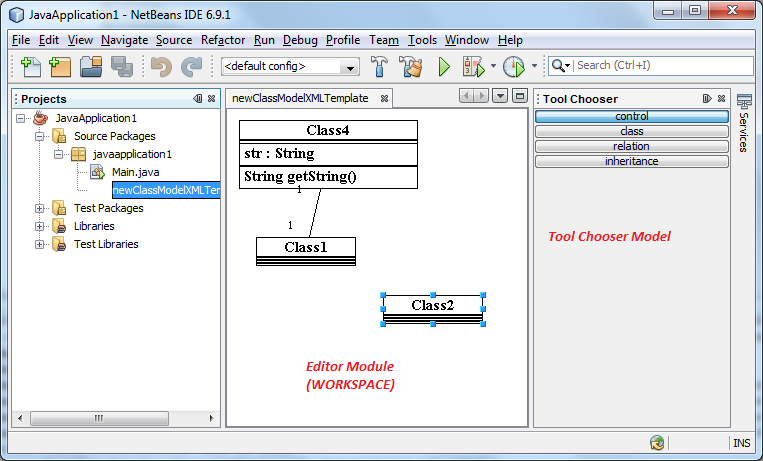
\includegraphics[width=\textwidth]{img/screenSmall.png}
\caption{Screenshot of the program}
\label{f-screenSmallModule}
\end{center}
\end{figure}

Figure \ref{f-Editor_ToolChooser_Components} illustrates the relation between Editor and ToolChooser modules. Editor provides instances of ToolChooserModel and IClassModelModel. These interfaces can be used by other modules. One (and maybe the once) of these modules is ToolChooser which uses ToolChooserModel to set the desired tool of active workspace (Editor module). These interfaces will be described in greater detail in following section.

\begin{figure}[!ht]
\begin{center}
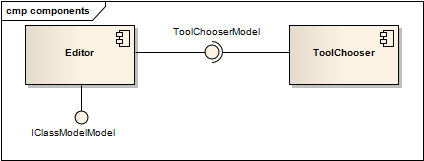
\includegraphics{img/Editor_ToolChooser_Components.png}
\caption{Component diagram of Editor and ToolChooser Modules}
\label{f-Editor_ToolChooser_Components}
\end{center}
\end{figure}

\section{API Module}

This module consists of Interfaces which implementations can be found in the lookup of the workspace (workspace is the part of the editor module). There are two packages in this module:

\begin{itemize}
    \item cz.cvut.indepmod.classmodel.api.model
    \item cz.cvut.indepmod.classmodel.api.toolchooser
\end{itemize}

\subsection{ClassModel API (cz.cvut.indepmod.classmodel.api.model)}

In this package there are interfaces which can be used to read the Class Model Notation Model. There is an implementation of the IClassModelModel interface in the workspace lookup. This object provides the list of Classes from a model. Classes provides the list of annotations, attributes, methods and relations to other classes. And so on with the attributes, etc. 

Relation between (two) classes is represented by instance of IRelation interface. IClass returns the list of IRelations that belongs to it. IRelation holds information about its type (simple relation, composition, agregation, generalization, implementation) and about what class is at the beginning and at the end of the relation, including cardinalities. 

Cardinalities are represented by instance of ICardinality interface. The ICardinality interface has two methods (getFrom() and getTo()) which return from and to value (both are of integer type). Sign of infinity (e.g. 1..* or *) is treated as -1. In the Table \ref{tab:cardinalityExamples} you can see examples of return values of some cardinalities.

\begin{table}[h]
\begin{center}
\begin{tabular}{|l|c|c|}
	\hline
	{ \bf Cardinality } & { \bf getFrom() result } & { \bf getTo() result } \\
	\hline \hline
	0 (or 0..0)      & 0 & 0  \\
	1 (or 1..1)      & 1 & 1  \\
   4 (or 4..4)      & 4 & 4  \\
	* (or 0..*)      & 0 & -1 \\
	1..*             & 1 & -1 \\
   0..1             & 0 & 1  \\
   2..5             & 2 & 5  \\
	\hline
\end{tabular}
\caption{Examples of cardinalities}
\label{tab:cardinalityExamples}
\end{center}
\end{table}

TODO: Image with structure (tree)

%The interface structure can be seen in the Figure \ref{f-ModuleAPIClassModelModelInterface}.

%\begin{figure}[!ht]
%\begin{center}
%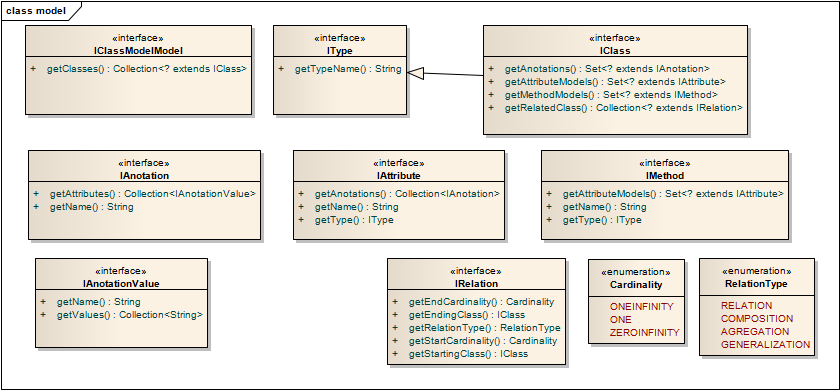
\includegraphics[width=\textwidth]{img/ModuleAPIClassModelModelInterface.png}
%\caption{Class Diagram of ClassModel API package}
%\label{f-ModuleAPIClassModelModelInterface}
%\end{center}
%\end{figure}

\subsection{ToolChooser API (cz.cvut.indepmod.classmodel.api.toolchooser)}

This package is used by both ToolChooser and Editor modules. Workspace (part of Editor Module) has an instance of ToolChooserModel in it's lookup. ToolChooser uses this instance (from the lookup of active workspace) to set the desired tool (e.g. new class). Structure is really simple and you can see it in the Figure \ref{f-ModuleAPIToolChooserModel}.

\begin{figure}[!ht]
\begin{center}
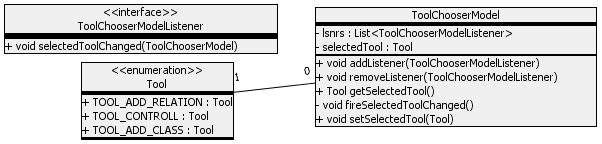
\includegraphics[width=\textwidth]{img/ModuleAPIToolChooserModel.png}
\caption{Class Diagram of ToolChooser API package}
\label{f-ModuleAPIToolChooserModel}
\end{center}
\end{figure}

\section{ToolChooser Module}

This module is used for setting of demanded tool of active workspace. The structure can be seen in the Figure \ref{f-ToolChooserModuleToolChooser}.

\begin{figure}[!ht]
\begin{center}
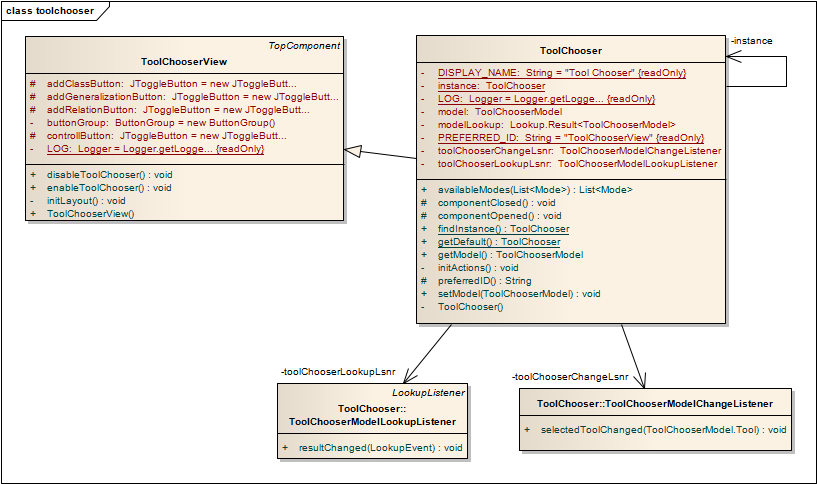
\includegraphics[width=\textwidth]{img/ToolChooserModuleToolChooser.png}
\caption{Class Diagram of ToolChooser Module}
\label{f-ToolChooserModuleToolChooser}
\end{center}
\end{figure}

ToolChooser is a singleton which is inherited from the TopComponent class. TopComponent is provided by Netbeans platform. Its ancestors can be used as a user interface (component that is visible to the user) in the application. TopComponent is derived from standard JComponent class (javax.swing) and adds many methods which can be used for controlling a window (more info in \cite{netbeans6.9DevGuide} in chapter called Window System).

ToolChooser searches for instance of the ToolChooserModel in the lookup of active workspace (Editor module). When the instance is found, ToolChooser can set its tool (class, relation, etc.). This means that it can be used to set the desired tool of that workspace.

In the layer.xml file there is set the action for opening the ToolChooser (Windows \ding{221} Tool Chooser).

\section{Editor Module}

This is the fundamental module whose purpose is to create a workspace where user can create a class model. For class modeling is used framework JGraph (http://www.jgraph.com/). More info about JGraph framework can be found in \cite{jgraphmanual}.

\subsection{Module Structure}

Main class (part of the cz.cvut.indepmod.classmodel.workspace package), which comprises the workspace, is the ClassModelWorkspace. Thus, if you want to study the code, you should start right here. ClassModelWorkspace is extended from the TopComponent. This class is responsible for whole initialisation. It creates:
\begin{itemize}
    \item ClassModelGraph - this class is extended from JGraph and represents the class model graph to the user. Instance of this class is situated inside the ClassModelWorkspace component (JGraph is also derived from JComponent)
    \item ClassModelModel - Implementation of IClassModelModel which returns the list of classes that are in the class model.
    \item ClassModelMarqueeHandler - this class is responsible for handling of user inputs that are made inside the ClassModelGraph.
    \item JPopupMenu - this popup menu is used inside the ClassModelGraph
\end{itemize}

ClassModelWorkspace is simply JComponent (TopComponent) which has the JGraph inside. JGraph presents the class model to the user. There are cells (representing classes) which are related together by edges (representing relations).

In next section I will try to describe the implementation of the Editor Module. I Will start from the initialization and after that I will try to explain every part that is created during the initialization.

\subsection{Editor Module Initialisation}

As I have already said before, the ClassModelWorkspace class do the initialization of the whole module. There are two cases of initialization. The first case, when user creates new class diagram, and the second, when user opens an existing file. Both cases are very similar. They differ only in the way of GraphLayoutCache initialization. For this purpose there are two constructor variants.

The first, non parametric, is used when the new class diagram (with no associated file) is created. This constructor creates new instance of GraphLayoutCache by ClassModelDiagramModelFactory.

The second constructor is used when the user opens a file with a class model. It accepts an instance of ClassModelXMLDataObject (one parameter). This object represents the file in which is the class model saved (more in the chapter \ref{subsection:fileAssociation}). The constructor gets the name (path) of that file and asks the ClassModelXMLCoder to decode its content. ClassModelXMLCoder decodes it and returns GraphLayoutCache instance filled according to that file's content. ClassModelXMLCoder is part of the persistence layer and will be discussed in the chapter \ref{subsection:persistence}.

%The second, which accepts ClassModelXMLDataObject instance, is used when there is a class model saved in a file. It finds out the name (path) of associated file and ask ClassModelXMLCoder for decoding. ClassModelXMLCoder decodes the file and returns loaded GraphLayoutCache (with all data).

After the GraphLayoutCache is gained (created or loaded) the initialization is the same. What the ClassModelWorkspace creates have been already written up. For better understanding you can see the sequence diagram in the Figure \ref{f-ClassModelWorkspaceInicializationSimple} which shows the initialisation of new ClassModelWorkspace. For simplicity there is only what ClassModelWorkspace creates. The processes inside these classes are not shown (Sequence diagram would have been really big) but it will be discussed later.

\begin{figure}[!ht]
\begin{center}
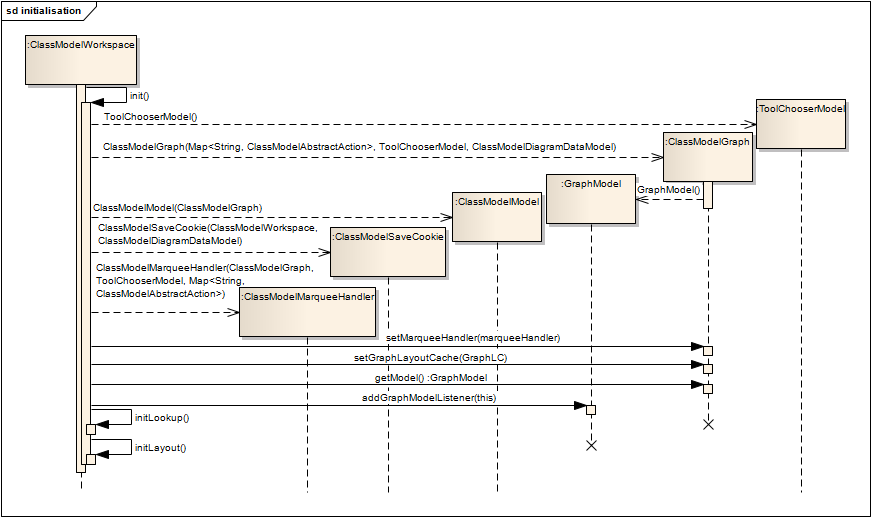
\includegraphics[width=\textwidth]{img/ClassModelWorkspaceInicializationSimple.png}
\caption{Simplified sequence diagram of ClassModelWorkspace initialization}
\label{f-ClassModelWorkspaceInicializationSimple}
\end{center}
\end{figure}

\subsection{Netbeans File Association}
\label{subsection:fileAssociation}

Netbeans platform allows its plug-ins to recognize new types of files. So when you want to associate new file type with your plugin, you can do it easily. If you are not familiar with this, you can find it in the \cite{netbeans6.9DevGuide} in the chapter called Data System.

%When user wants to create new class diagram, he has to have an opened project. Then he simply adds new class diagram file (Other \ding{221} Empty ClassModelXML file) into this project.

The file type association settings can be found in layer.xml file. This file is used for settings of Netbeans module. At present there is settings of action that opens new class diagram without associated file, file type association and settings of template that can be used to create new class diagram file. Files that are associated with this plugin are xml files with .cls suffix. Content of the file will be discussed later.

\subsection{ClassModelGraph implementation}

ClassModelGraph is extended from JGraph and adds some functionality for Class manipulation. Added methods are:
\begin{itemize}
    \item insertCell(Point p) - creates new cell on desired position according to the selected tool (in ToolChooserModel). Usage of this function is shown in the section \ref{subsection:apiImplementation} in Figure \ref{f-ClassCreationSequenceDiagram}.

    \item getAllClasses() - returns the list of classes that are in the diagram. Usage of this function will be shown in the section \ref{subsection:apiImplementation}

    \item getAllTypes() - returns the list of all data types in the diagram. In addition to the classes (the class is a data type) there are also static data types (like String or int in Java).
\end{itemize} 

For event handling in the graph (ClassModelGraph) there is the ClassModelMarqueeHandler. Instance of this class is created in the ClassModelWorkspace and is added into the ClassModelGraph instance. Purpose of this class is to handle all user inputs in the ClassModelGraph (in the canvas of the graph). When user does an action (e.g. click with mouse), the ClassModelMarqueeHandler will find out if it is a control click (e.g. cell selection), new cell addition, edge (line between cells) addition and so on. This class is also responsible for rendering of the temporary line when user creates new edge.

\subsection{ClassModel API implementation}
\label{subsection:apiImplementation}

Implementation classes of ClassModel API (its interfaces are in the API Module) are situated in the cz.cvut.indepmod.classmodel.cell.model.classmodel package. Main problem I had to deal with was to design where to store the data of the ClassModel.

Basically, ClassModel class is used as a User Object for JGraph cells. User Object (Class Model instance) does not have normally the pointer to its cell (only cell has the pointer to it's User Object). ClassModel holds information like name of the class and list of its attributes, methods and annotations. But where to store the information about relations with other cells (classes)? This information is stored in the JGraph (in its model). So the first idea was to copy this information into the ClassModel instance when an relation is created. But this is not very nice because of data duplication. The second purpose was to add an pointer to cell into the ClassModel instance. But how? The answer is quite simple. I created the ClassModelClassCell which extends DefaultGraphCell of JGraph. The extension of this class is that it adds an pointer to itself into the User Object if this User Object is instance of ClassModel.

So problem is solved. Some information like the name are stored inside the User object and some like the relations are gained from the JGraph cell. In the Figure \ref{f-ClassCreationSequenceDiagram} you can see how is created a class when user selects new class tool in the ToolChooser and clicks somewhere in the ClassModelGraph (JGraph) workspace.

\begin{figure}[!ht]
\begin{center}
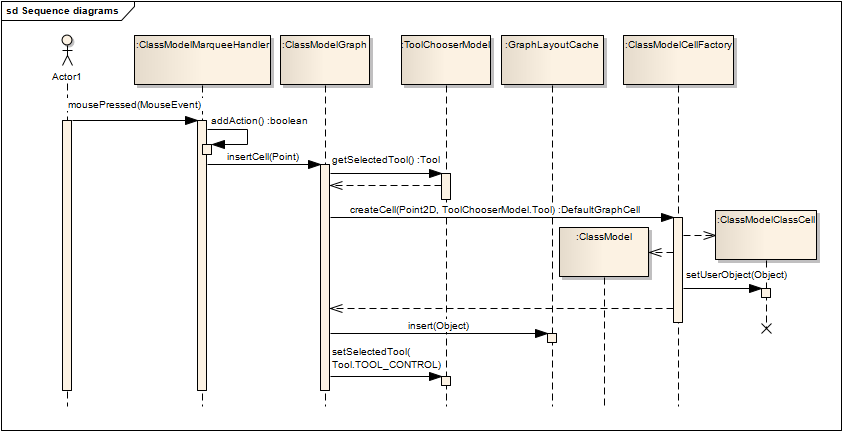
\includegraphics[width=\textwidth]{img/ClassCreationSequenceDiagram.png}
\caption{Sequence Diagram of class creation}
\label{f-ClassCreationSequenceDiagram}
\end{center}
\end{figure}

\subsection{JGraph class cell rendering}

%In this section I will explain how I render the class (the rectangle with the class name and lists of annotations, attributes and methods) into the JGraph workspace. JGraph basically supports rendering of basic shapes like rectangles, ovals and so on. When you want to render your own shape, you have to create your own CellViewFactory implementation which will create your own VertexView. VertexView provides, among other things, the CellViewRenderer and it returns a Component (java.awt) which can be printed into the JGraph workspace. More on this theme can be found in \cite{jgraphmanual}.

In this section I will explain how I render the class (the rectangle with the class name and lists of annotations, attributes and methods) into the JGraph workspace. But first a little theory remind. JGraph uses MVC pattern for cell rendering. Cells (the model of cell) in JGraph are represented by DefaultGraphCell (or its subclasses). DefaultGraphCell implementation stores the user object and an attribute map inside which is used when you want to set the appearance of that cell. All graph cell has an associated view (VertexView implementation). This VertexView implementation associates the renderer, editor and cell handle together for an cell (DefaultGraphCell implementation). The cell and view is associated together by CellViewFactory which returns a cell view for a particular cell. More on this theme can be found in \cite{jgraphmanual}.

JGraph basically supports rendering of basic shapes like rectangles, ovals and so on. When you want to render your own shape, you have to create your own cell view (VertexView), renderer (CellViewRenderer) and CellViewFactory implementation.

% JGraph VertexView provides, among other things, the CellViewRenderer and it returns a Component (java.awt) which can be printed into the JGraph workspace. More on this theme can be found in \cite{jgraphmanual}.

%So this is exactly what I did. I created ClassModelCellViewFactory which is derived from JGraph's DefaultCellViewFactory and overrides it's method createVertexView(Object o). This method returns new instance of ClassModelVertexView (derived from JGraph's VertexView). ClassModelVertexView returns statically instantiated ClassModelVertexRenderer which is derived from VertexRenderer and overrides method getRendererComponent(...). This method returns new instance of ClassComponent if the User Object of the cellView (argument) is of ClassModel type. ClassComponent is extended from JComponent and renders the class according to the ClassModel user object.

So this is exactly what I did. I created ClassModelCellViewFactory which is derived from JGraph's DefaultCellViewFactory and overrides it's method createVertexView(Object o). If the object in the parameter is instance of ClassModelClassCell class, the method returns new instance of ClassModelVertexView (derived from JGraph's VertexView). Otherwise the method returns the default view (calls its parent's method). ClassModelVertexView returns statically instantiated ClassModelVertexRenderer which is derived from VertexRenderer and overrides its method getRendererComponent(...). This method returns new instance of ClassComponent if the User Object of the cellView (argument) is of ClassModel type. ClassComponent is extended from JComponent and renders the class according to the ClassModel user object.

These classes can be found in the package cz.cvut.indepmod.classmodel.workspace.cell. Instance of ClassModelCellViewFactory is inserted into the GraphLayoutCache during the workspace initialisation. You can see the class diagram in the Figure \ref{f-ClassModelVertexStructure}.

\begin{figure}[!ht]
\begin{center}
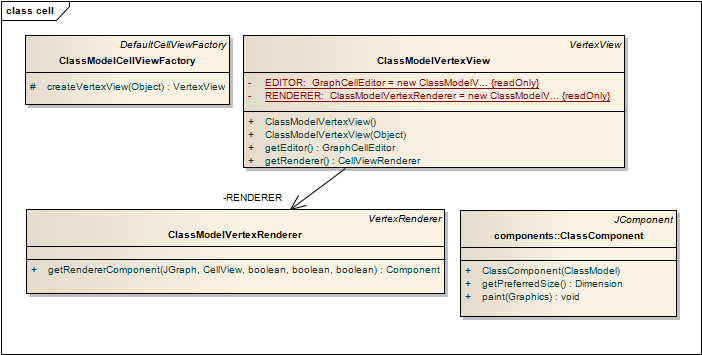
\includegraphics[width=\textwidth]{img/ClassModelVertexStructure.png}
\caption{Structure of classes which render the class cell}
\label{f-ClassModelVertexStructure}
\end{center}
\end{figure}

\subsection{Persistence}
\label{subsection:persistence}

Persistence layer implementation is situated in the cz.cvut.indepmod.classmodel.persistence.xml package. There is a ClassModelXMLCoder class that is created as a singleton. Instance of this class is responsible for encoding and decoding the GraphLayoutCache instance into or from a file. Its method for encoding, encode(GraphLayoutCache cache, String filename), is called by SaveCookie (discussed in the section \ref{subsection:lookup}).

ClassModelXMLCoder uses java.beans.XMLEncoder and java.beans.XMLDecoder. This creates the xml file that represents the steps to create the exactly same object that was encoded. Because XMLEncoder can encode in default only some types of objects, there are some persistence delegates that allow to encode particular object I use. These persistence delegates can be found in the cz.cvut.indepmod.classmodel.persistence.xml.delegate package.

If you want to know more about how XMLEncoder or XMLDecoder works, please take a look at \cite{usingXMLEncoder}.

\subsection{Lookup}
\label{subsection:lookup}

Lookup is (in Netbeans platform) a technique to join more plugins together with loose coupling. On the module level, lookups enable to register a service by its provider and find the service by its consumer. On the level of single components (TopComponent), lookups enable to exchange data between this component (provider) and consumers. More reading about this can be found in \cite{netbeans6.9DevGuide} in the chapter called Lookup.

Editor Module uses the Lookup on the component level. ClassModelWorkspace creates its Lookup during the initialization. It adds there an instance of ToolChooserModel and an instance of ClassModelModel.

ToolChooserModel instance is used by ToolChooser Module to set the desired tool. Thanks to this, there can be one ToolChooser component which manages all ClassModelWorkspaces. Of cource, ToolChooserModel instance in the lookup can be used by other plugins also.

ClassModelModel instance implements the IClassModelModel interface and can be also used by other plugins. It provides the Class Model API to the outside world. Thanks to this there can be for example another plugin that will generate the code from the class model of this module.

When user does any change into the model (add new class, new relation between classes, change the attribute of the class or something similar), ClassModelWorkspace inserts an SaveCookie instance into its Lookup. This tells the Netbeans platform that this component is changed and can be saved (save action in File menu is enabled). When user calls this action, the SaveCookie tells the ClassModelXMLCoder to save the GraphLayoutCache into the associated file. When it is done, this SaveCookie implementation is removed from the Lookup, so the Netbeans platform knows that the component does not have to be saved.

\subsection{Package Structure}

You can see the package structure in this directory tree:
\renewcommand*\DTstylecomment{\rmfamily\color{black}\textsc}
\renewcommand*\DTstyle{\ttfamily\textcolor{blue}}
\dirtree{%
.1 cz.cvut.indepmod.classmodel.
.1 actions\DTcomment{Actions for buttons etc.}.
.1 file\DTcomment{SaveCookie and file type association support}.
.1 frames.
.2 dialogs.
.1 modelfactory.
.2 diagrammodel.
.1 persistence\DTcomment{layer for data saving}.
.2 xml\DTcomment{implementation of persistence for saving into a XML file}.
.3 delegate\DTcomment{XML Delegates for mapping into xml}.
.1 resources.
.1 workspace\DTcomment{Main package containing the TopComponent with JGraph}.
.2 cell\DTcomment{Cells, renderers, VertexViews, etc. for JGraph}.
.3 components\DTcomment{Component for JGraph}.
.3 model.
.4 classmodel\DTcomment{Implementation of ClassModel API from API Module}.
}
\parindent=\luckyparindent

\begin{thebibliography}{9}
\bibitem{jgraphmanual}{\it{JGraph 5 manual}, found at \texttt{http://www.jgraph.com/downloads/jgraph/jgraphmanual.pdf}}

\bibitem{netbeans6.9DevGuide}{PETRI, J�rgen. \it{NetBeans Platform 6.9 	Developer's Guide}. Birmingham : Packt Publishing Ltd., 2010. 273 s. ISBN 978-1-849511-76-6}

\bibitem{usingXMLEncoder}{MILNE, Philip. Sun Developer Network [online]. c2010 [cit. 2011-01-29]. Using XMLEncoder. Available from WWW: <http://java.sun.com/products/jfc/tsc/articles/persistence4/>.}
\end{thebibliography}

\end{document}

\end{document}

